%\chapter*{Неделя 1}
\protect\thispagestyle{fancy}
\section{}
Изобразить на одном чертеже модули спектров двух последовательностей c одинаковым периодом $T$.
Указать значение максимальной спектральной плотности.

\begin{figure}[!h]
	\centering
	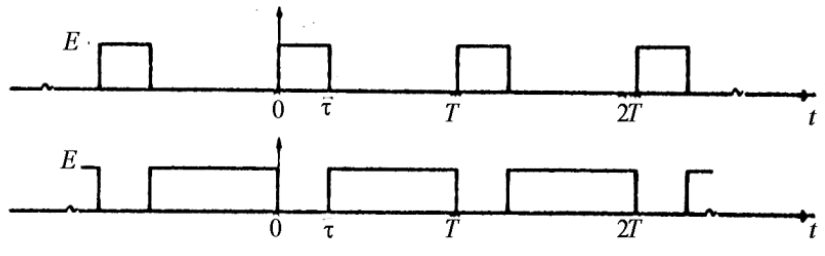
\includegraphics[width=0.6\columnwidth]{pics/fall/1/x.png}
\end{figure}

Огибающие спектров этих последовательностей:
\begin{align*}
	\widetilde{\Capit{X}}_1(\omega) &= \int \limits_{0}^{T} \s{x}_1(t)e^{-j \omega t} dt =
	E \int \limits_{0}^{\tau} e^{-j \omega t} dt = \frac{E}{-j \omega} \Big(e^{-j \omega \tau} - 1 \Big)
	=\\&= \frac{2 E}{\omega} e^{-j \frac{\omega \tau}{2}} \Bigg(\dfrac{e^{+j \frac{\omega \tau}{2}} - e^{-j \frac{\omega \tau}{2}}}{2 j} \Bigg) = ET \frac{\tau}{T} e^{-j \frac{\omega \tau}{2}} \cdot \sinc\Big(\frac{\omega \tau}{2}\Big).\\
	\widetilde{\Capit{X}}_2(\omega) &= \int \limits_{0}^{T} \s{x}_2(t)e^{-j \omega t} dt =
	E \int \limits_{\tau}^{T} e^{-j \omega t} dt 
	= \frac{E}{-j \omega} \Big(e^{-j \omega T} - e^{-j \omega \tau} \Big)
	=\\&= \frac{2 E}{\omega} e^{-\frac{j\omega}{2}(T + \tau)} \Bigg(\dfrac{e^{+\frac{j\omega}{2}(T - \tau)} - e^{-\frac{j\omega}{2}(T - \tau)}}{2 j} \Bigg) = ET \Big(1 - \frac{\tau}{T}\Big) e^{-\frac{j \omega}{2}(T + \tau)} \cdot \sinc\Big(\frac{\omega (T - \tau)}{2}\Big).
\end{align*}

\begin{figure}[!h]
	\centering
	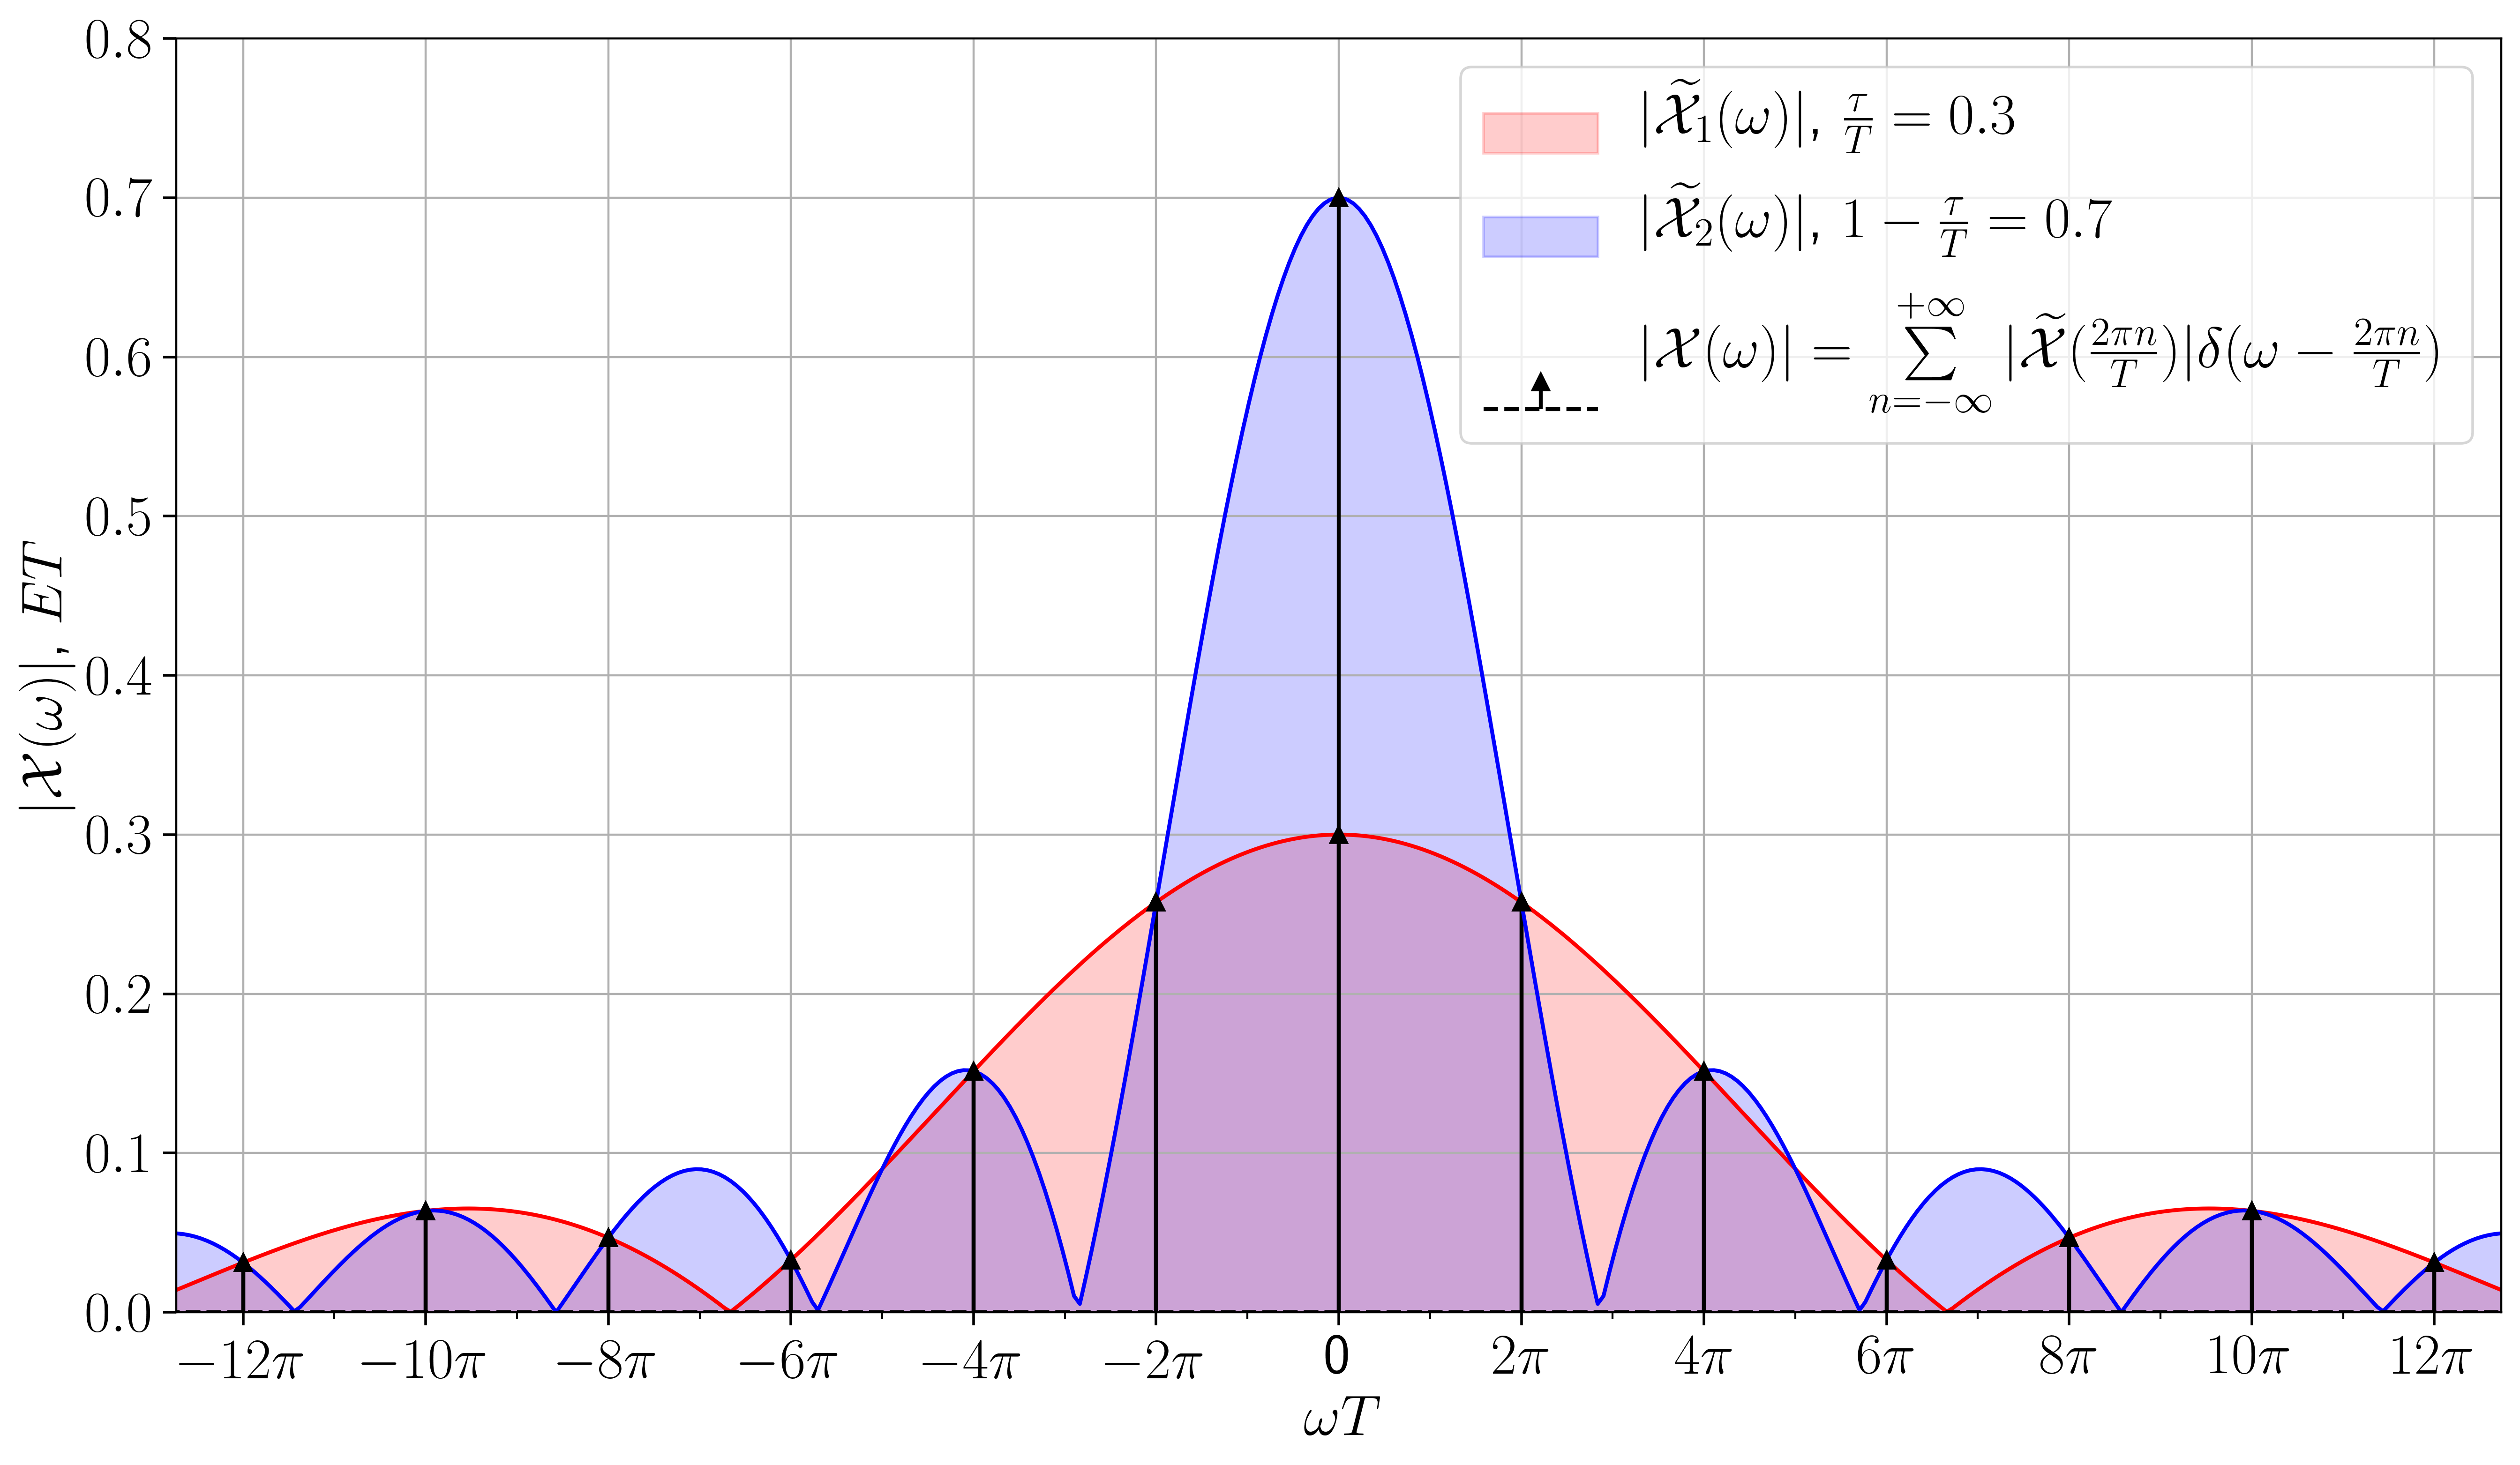
\includegraphics[width=0.95\columnwidth]{pics/fall/1/1-1.png}
	\label{fig:1}
\end{figure}

Максимальные значения спектральной плотности достигаются при $\omega = \omega_n = 0$, пропорциональны параметру скважности и соответственно равны $ET\cdot \frac{\tau}{T}$, $ET\cdot \Big( 1 - \frac{\tau}{T} \Big)$.



\section{}
Определить спектр окна Ханна длительностью $\tau = 2T$:
\begin{equation*}
	\s{w}(t) = 
	\begin{cases}
		\frac{1}{2} \Big(1 + \cos\big(\frac{\pi t}{T}\big) \Big) = \frac{1}{2} + \frac{1}{4} \Big(e^{-j\frac{\pi t}{T}} + e^{j\frac{\pi t}{T}}\Big),&\text{если } |t|< T\\
		0,&\text{если } |t|\geq T
	\end{cases}.
\end{equation*}

Найти отношение уровней первого бокового и главного лепестков.

\begin{align*}
	&\Capit{W}(\omega) = \int \limits_{-\infty}^{+\infty} \s{w}(t) e^{-\s{j} \omega t} dt = 
	\frac{1}{2} \int \limits_{-T}^{+T} e^{-\s{j} \omega t} dt + 
	\frac{1}{4} \int \limits_{-T}^{+T} e^{-\s{j} (\omega + \frac{\pi}{T}) t} dt + 
	\frac{1}{4} \int \limits_{-T}^{+T} e^{-\s{j} (\omega - \frac{\pi}{T}) t} dt =\nonumber\\
	&=\frac{1}{2} \Capit{D}_{T}(\omega) + \frac{1}{4}\Capit{D}_{T}\big(\omega + \frac{\pi}{T}\big) + \frac{1}{4}\Capit{D}_{T}\big(\omega - \frac{\pi}{T}\big) \footnotemark  =\dfrac{\sin(\omega T)}{\omega} + \frac{T}{2} \dfrac{\sin(\omega T + \pi)}{(\omega T + \pi)} + \frac{T}{2} \dfrac{\sin(\omega T - \pi)}{(\omega T - \pi)}=\\
	&=\dfrac{\sin(\omega T)}{\omega} - \frac{T}{2} \dfrac{\sin(\omega T)}{(\omega T + \pi)} - \frac{T}{2} \dfrac{\sin(\omega T)}{(\omega T - \pi)} = \dfrac{- (\pi T)^2 sin(\omega T)}{\omega T ((\omega T)^2 - \pi^2)}.
\end{align*}

\footnotetext{$\Capit{D}_T(\omega)$ -- спектр прямоугольного окна длительностью $\tau=2T$.}

\begin{align*}
	&\dfrac{d \Capit{W}(\omega)}{d\omega} = 0, \quad \Rightarrow \omega \in \{0, \pm 7.4202, \pm 10.706, \pm 13.9175, \ldots\}. \\
	&\Bigg| \dfrac{\Capit{W}(\omega_1)}{\Capit{W}(\omega_0)} \Bigg|^2 = \Big| \Capit{W}(7.4202) \Big|^2 = 0.02671^2 = 0.0007133 = -31.47\text{ dB}.
\end{align*}


\begin{figure}[!h]
	\centering
	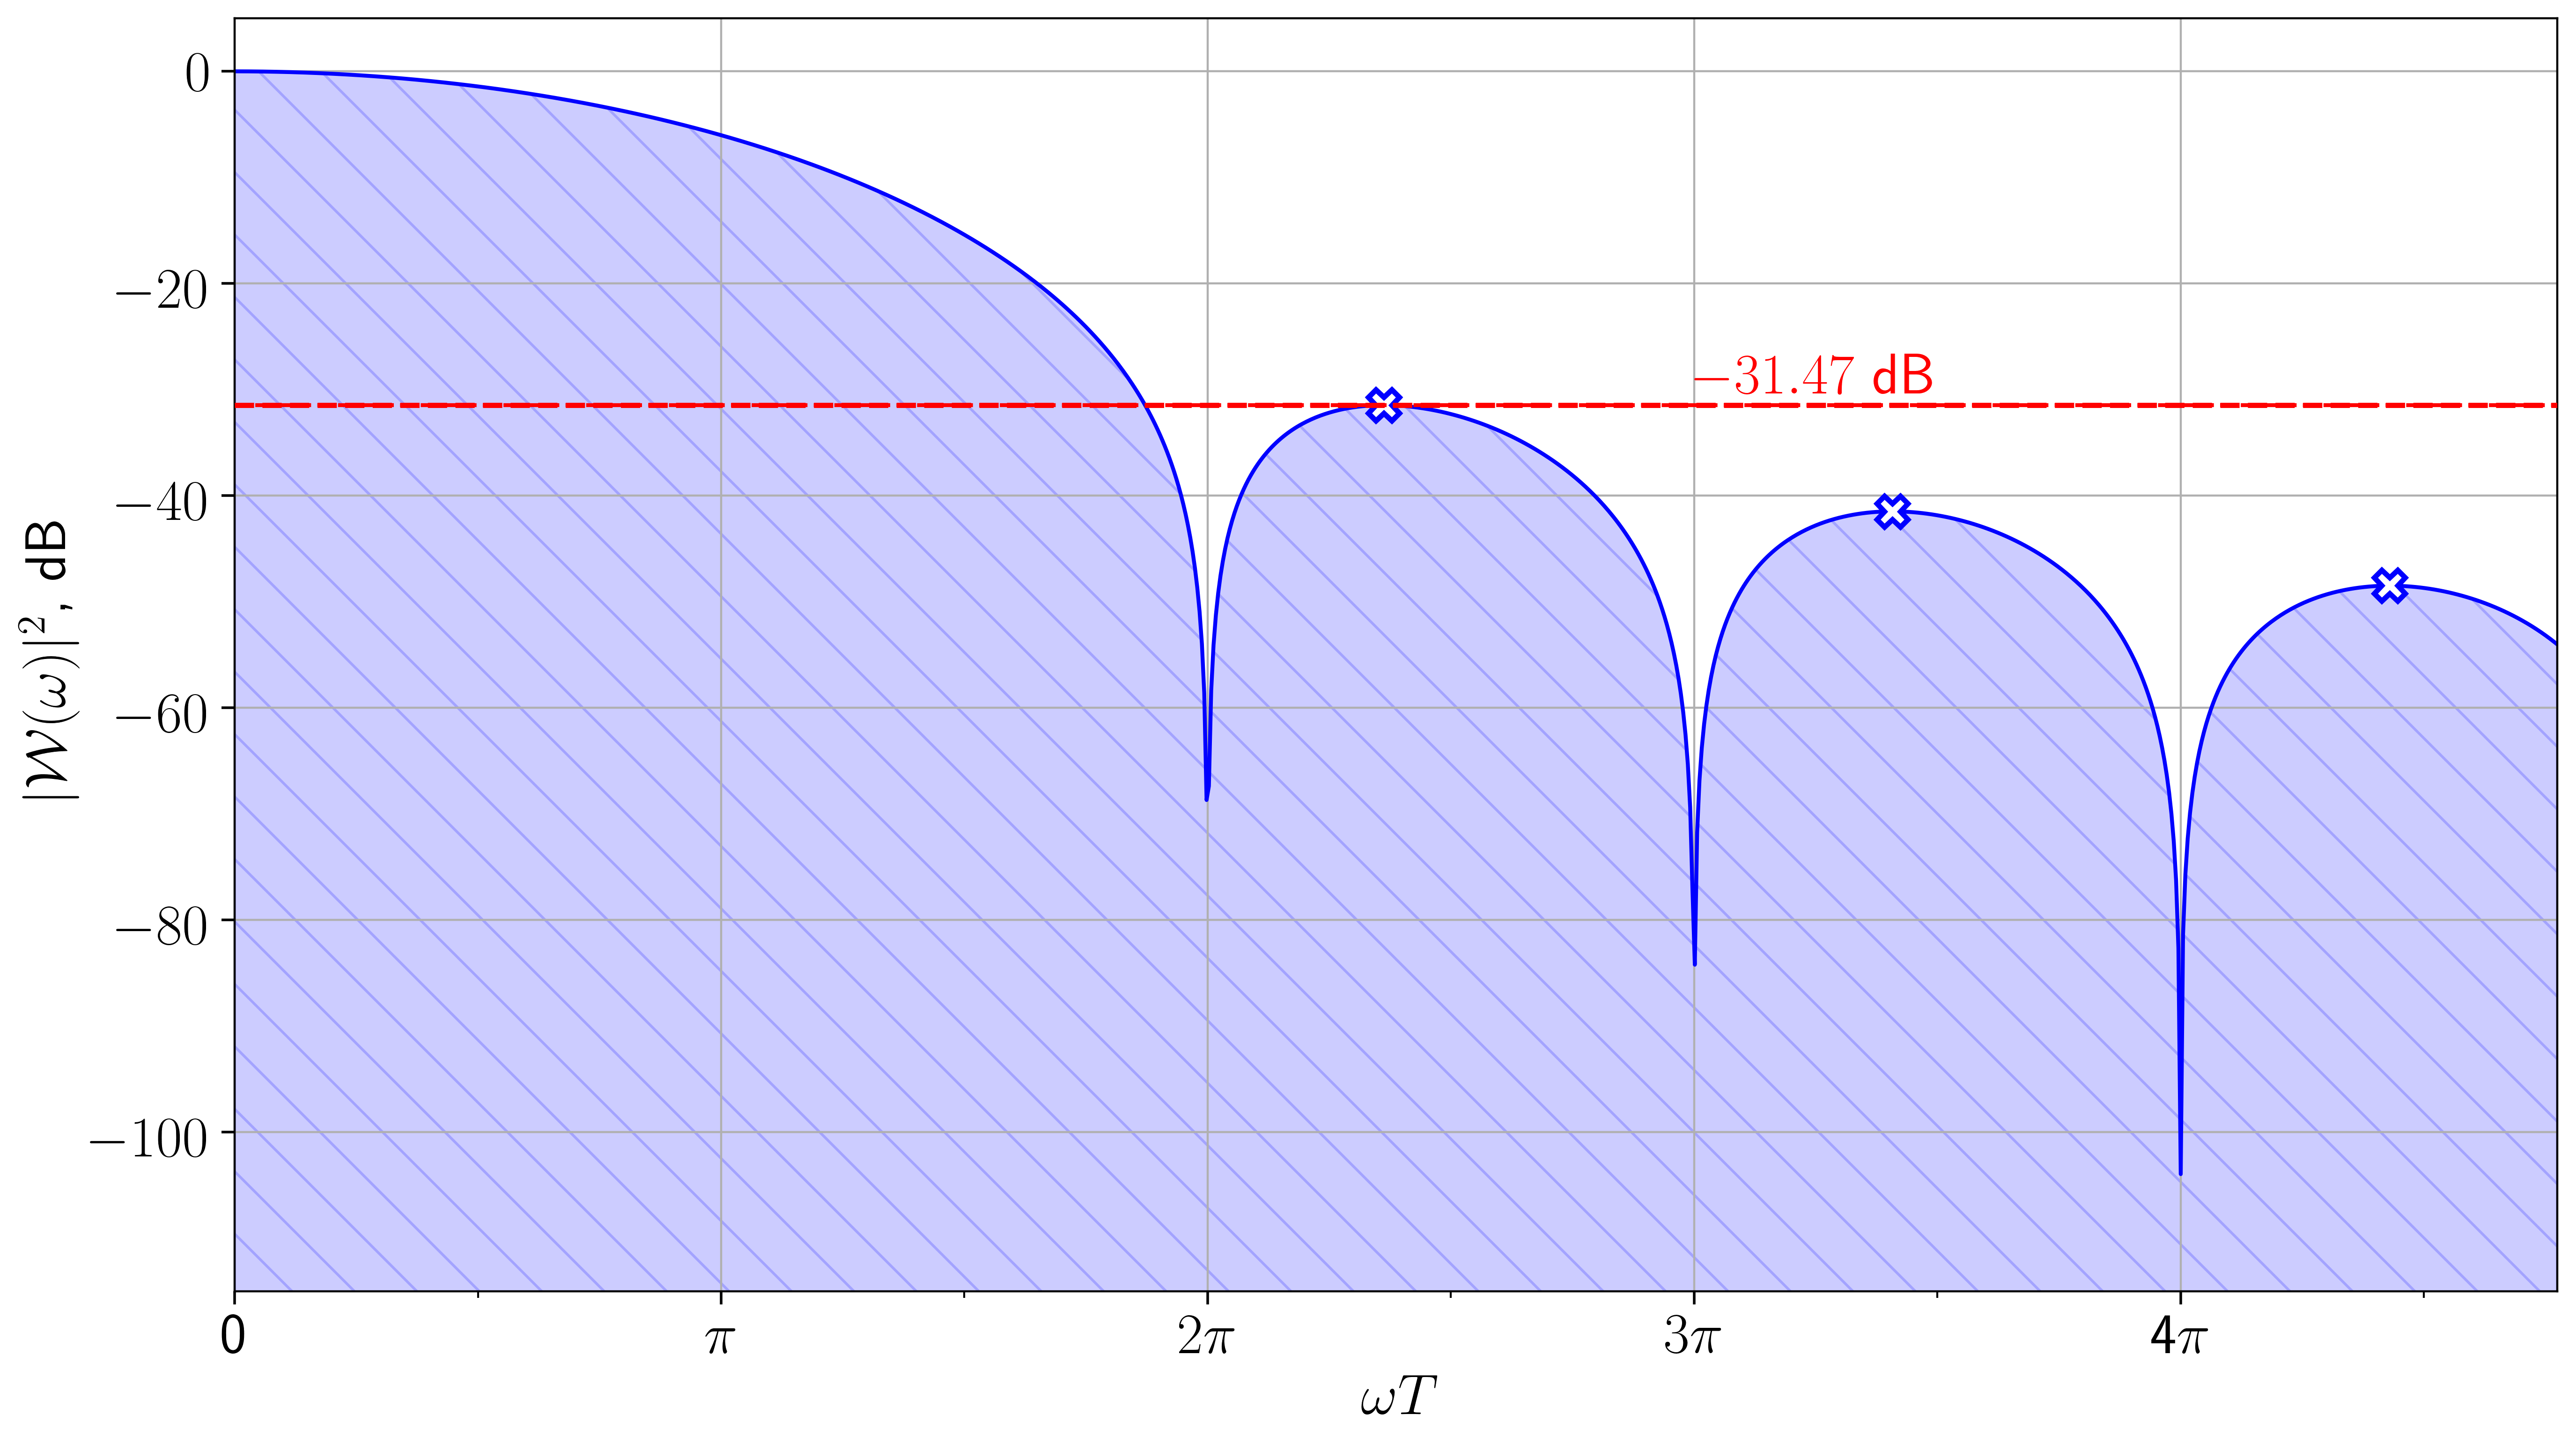
\includegraphics[width=0.95\columnwidth]{pics/fall/1/1-2.png}
	\caption{Спектр окна Ханна.}
	\label{fig:topology}
\end{figure}


\section{}
Найти спектр функции отсчетов, используемых в теореме Котельникова.

\begin{equation*}
	\phi_k(t) = \dfrac{\sin(2\pi f_B(t - k \Delta t))}{2\pi f_B(t - k \Delta t)},\quad \Delta t = \dfrac{1}{2f_{B}}.
\end{equation*}


Доказать их ортогональность, используя равенство Парсеваля для прямоугольного импульса и дуализм времени и частоты преобразовании Фурье.

\begin{align*}
	&\Phi_k(f) = \int \limits_{-\infty}^{+\infty} \phi_k (t) e^{-j 2\pi f t} dt = \int \limits_{-\infty}^{+\infty} \dfrac{\sin(2\pi f_B(t - k \Delta t))}{2\pi f_B(t - k \Delta t)} e^{-j 2\pi f t} dt = 
	\dfrac{e^{j 2\pi f k \Delta t}}{2\pi f_B}\int \limits_{\infty}^{+\infty} \textcolor{blue}{\dfrac{\sin(\s{u})}{\s{u}}} e^{-j \s{u} \frac{f}{f_B}} d\s{u} =\\
	&= \dfrac{e^{j 2\pi f k \Delta t}}{2\pi f_B}\int \limits_{\infty}^{+\infty} \textcolor{blue}{\Big(\int \limits_{-1}^{+1} \frac{1}{2} e^{j \s{uv}} d \s{v} \Big)} e^{-j \s{u} \frac{f}{f_B}} d\s{u} = 
	\frac{1}{2}  \dfrac{e^{j 2\pi f k \Delta t}}{2\pi f_B} \int \limits_{-1}^{+1} d \s{v} \textcolor{red}{\int \limits_{-\infty}^{\infty} e^{j (\s{v} - \frac{f}{f_B}) \s{u}} d \s{u}} = 
	\frac{1}{2}  \dfrac{e^{j 2\pi f k \Delta t}}{2\pi f_B} \int \limits_{-1}^{+1} d \s{v} \cdot \textcolor{red}{2 \pi \delta \Big(\s{v} - \frac{f}{f_B}\Big)} =\\
	&= \pi \dfrac{e^{j 2\pi f k \Delta t}}{2\pi f_B} \Bigg[\Theta \Big(1 - \frac{f}{f_B} \Big) - \Theta \Big(- 1 - \frac{f}{f_B} \Big) \Bigg] = 
	\pi \dfrac{e^{j 2\pi f k \Delta t}}{2\pi f_B} \Bigg[\Theta \Big( f + f_{B}\Big) - \Theta \Big(f - f_B\Big) \Bigg].
\end{align*}

Согласно равенству Парсеваля:
\begin{align*}
	\braket{\phi_k|\phi_n} &= \int \limits_{-\infty}^{+\infty} \phi_k(t)\phi_n(t)dt 
	= \int \limits_{-\infty}^{+\infty} \Phi_k(f) \Phi_n^*(f) df = 
	\dfrac{\pi^2}{(2 \pi  f_B)^2} \int \limits_{-f_B}^{f_B} e^{j2\pi f (k - n) \Delta t} df = \\
	&= \dfrac{\pi^2}{(2 \pi  f_B)^2} \dfrac{e^{j2\pi f_B (k - n) \Delta t} - e^{-j2\pi f_B (k - n) \Delta t}}{j2 \pi (k - n) \Delta t} = 
	\dfrac{\pi^2}{(2 \pi  f_B)^2} \dfrac{\sin(2\pi f_B (k - n) \Delta t)}{\pi (k - n) \Delta t} = 
	\dfrac{\sin(\pi (k - n))}{2 \pi  f_B (k - n)} = 0.\\
	\braket{\phi_k|\phi_k} &= \dfrac{\pi^2}{(2 \pi  f_B)^2} \int \limits_{-f_B}^{f_B} e^{j2\pi f (k - k) \Delta t} df =
	\dfrac{1}{2 f_B} = \Delta t.
\end{align*}

\begin{equation*}
	\boxed{\braket{\phi_k|\phi_n} = \delta_{kn} \Delta t. }
\end{equation*}

